% Compile with: pdflatex 3_10_Alejandro_DeLaTorre.tex
% (or) latexmk -pdf 3_10_Alejandro_DeLaTorre.tex

\documentclass[11pt]{beamer}

\usetheme{default}
\usepackage{graphicx}
\usepackage{hyperref}

\title{Regulatory Acceleration and the Composition of FDA Approvals}
\subtitle{Progress Report \#2: Pivot to Controlled-Substance Approvals}
\author{Alejandro De La Torre}
\institute{ECON 580}
\date{March 10, 2026}

\begin{document}

\begin{frame}
  \titlepage
\end{frame}

\begin{frame}{Pivot and New Research Questions}
\begin{itemize}
  \item \textbf{Old direction:} ``Faster FDA approval $\rightarrow$ diversion risk'' was too diffuse and hard to identify cleanly.
  \item \textbf{Primary question:} Did \textbf{PDUFA (1992)} increase approvals of \textbf{controlled substances}?
  \item \textbf{Secondary question:} Are \textbf{expedited review programs} disproportionately used for controlled substances?
  \item \textbf{Why this is stronger:} PDUFA is a policy shock, and controlled-substance status is an observable outcome.
\end{itemize}
\end{frame}

\begin{frame}{Motivation and Mechanism}
\begin{itemize}
  \item \textbf{PDUFA}: user fees + review deadlines + expanded FDA capacity \ $\Rightarrow$ faster approvals.
  \item Existing work asks: \textbf{speed vs. safety} and launch timing.
  \item My pivot asks: did regulatory acceleration change \textbf{which types of drugs} enter the market?
  \item Controlled substances are a policy-relevant category with clear legal classification.
\end{itemize}
\end{frame}

\begin{frame}{What the Literature Already Does}
\textbf{A) FDA speed / safety / PDUFA}
\begin{itemize}
  \item PDUFA and approval speed / safety tradeoffs (Philipson et al., 2008; Carpenter et al., 2008; Olson, 2008, 2009).
  \item Drugs reaching market sooner and launch timing (Dranove \& Meltzer, 1994; Olson, 2009).
\end{itemize}

\vspace{0.5em}
\textbf{B) Institutional FDA history}
\begin{itemize}
  \item Descriptive regulatory history (Darrow et al., 2020).
\end{itemize}

\vspace{0.5em}
\textbf{C) Supply-side drug policy / substitution}
\begin{itemize}
  \item Supply shocks and substitution in opioid markets (Alpert, Powell \& Pacula, 2018; Powell \& Pacula, 2021; Dobkin \& Nicosia, 2009).
\end{itemize}
\end{frame}

\begin{frame}{What Is New in This Project}
\begin{itemize}
  \item Existing work focuses on \textbf{speed vs. safety} and post-market outcomes.
  \item I focus on whether \textbf{regulatory acceleration changes composition} of approvals.
  \item Outcome is \textbf{controlled-substance status}, a clean, policy-relevant classification.
  \item Secondary contribution: whether expedited pathways are used disproportionately for drugs with abuse potential.
\end{itemize}
\end{frame}

\begin{frame}{What I Have Explored So Far (Preliminary)}
\begin{columns}
  \column{0.5\textwidth}
  \centering
  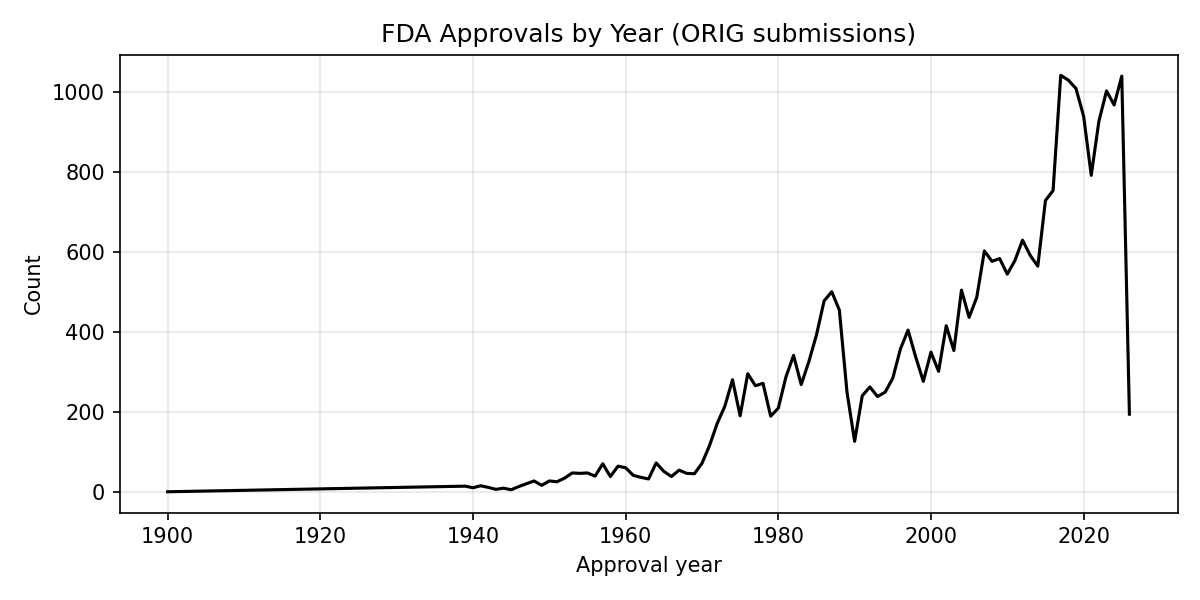
\includegraphics[width=\linewidth]{../../output/figures/approvals_by_year.png}
  \\
  {\scriptsize FDA approvals by year (Drugs@FDA).}

  \column{0.5\textwidth}
  \centering
  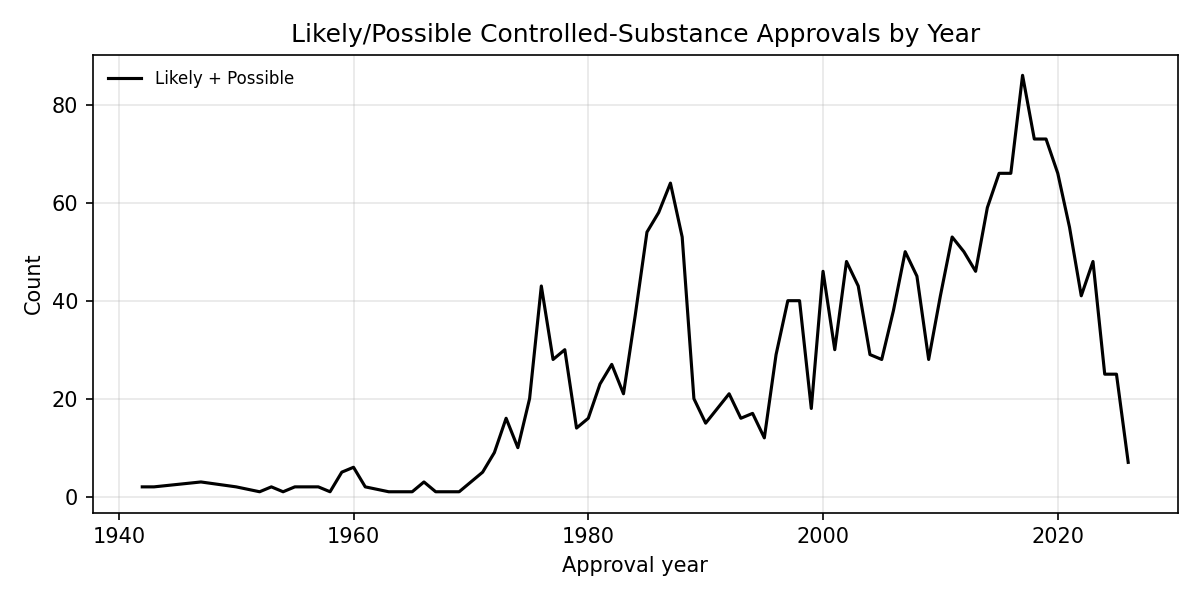
\includegraphics[width=\linewidth]{../../output/figures/controlled_substance_candidates_by_year.png}
  \\
  {\scriptsize Controlled-substance \emph{candidates} by year.}
\end{columns}

\vspace{0.5em}
{\scriptsize \textbf{Note:} controlled-substance classification is currently a \emph{heuristic screen} based on ingredient names; DEA schedule validation is pending.}
\end{frame}

\begin{frame}{Working Empirical Strategy (Draft)}
\begin{itemize}
  \item \textbf{Unit of observation:} drug-level FDA approvals over time (ORIG submissions).
  \item \textbf{Main outcome:} count/share/probability of controlled-substance approvals pre- vs post-PDUFA.
  \item \textbf{Secondary outcome:} expedited review usage within controlled substances.
  \item \textbf{Planned Figure 1:} controlled-substance approvals over time with PDUFA marked.
  \item \textbf{Planned Table 1:} summary by era and review designation.
\end{itemize}
\end{frame}

\begin{frame}{Main Concerns / Open Identification Questions}
\begin{itemize}
  \item How should ``controlled substance'' be defined consistently over time (DEA schedules I--V vs subset)?
  \item Best comparison: levels, shares, or approval probabilities?
  \item How to handle changes in therapeutic mix over time?
  \item Should the framing be ``PDUFA increased controlled-substance approvals'' or ``PDUFA changed composition''?
  \item What is the minimal defensible identification strategy for this class of question?
\end{itemize}
\end{frame}

\begin{frame}{Next Steps + Feedback}
\textbf{Next steps (next 2--4 weeks):}
\begin{enumerate}
  \item Build validated FDA $\times$ DEA schedule match.
  \item Refine descriptive figures and summarize by pre/post PDUFA eras.
  \item Decide final outcome metric (counts vs shares vs probabilities).
  \item Draft empirical design and outline data limitations.
\end{enumerate}

\vspace{0.75em}
\textbf{Feedback request:}
\begin{itemize}
  \item Is the pivot persuasive and the contribution clear?
  \item Which controlled-substance definition is most credible for this question?
  \item Are there key papers or data pitfalls I should address early?
\end{itemize}

\vspace{0.5em}
\textit{Comments and feedback welcome.}
\end{frame}

\end{document}
